\subsection{Evaluation of camera data}
\subsubsection{Object detection and preparation}
The first problem to deal with is to detect any possible object in every given frame. For that pyimagesearche published an useful version of a detection algorithm called \ac{YOLO} \cite{Yolo}. 
Changes in the code had to be made to use multiple frames instead of just one saved image stored on disk.
These frames of the simulation environment can be generated by in\,-\,game sensors like RGB \& depth camera. It is necessary to place those cameras at the same spot on the ego\,-\,vehicle to collect comparable images without any errors by considering angular misalignment. As a result, the camera\,-\,sensors will create images of 32\,-\,bit BGRA colours to work with. 
Because the \ac{YOLO} algorithm needs at least 0.35 seconds on all tested devices the tick rate has to be synchronized and reduced to 0.5 seconds for both sensors.

To generate predominantly \ac{TP} cases, the confidence value of \ac{YOLO} is set to 0.7 and the threshold value to 0.6. Furthermore, tests in Carla have resulted in \ac{FP} cases where objects such as umbrellas were detected. To exclude these cases, all irrelevant objects are filtered out in advance. The bounding boxes are not used as usual to display them in the frame, but the pixel coordinates of the bounding boxes are used. These are composed of an \textit{x and y coordinate}, as well as a \textit{width w} and \textit{height h} to determine the location of the detected object in the frame. In addition, the confidence and name of the detected objects are also used. 
\subsubsection{Data processing}
The resulting pixel coordinates of the bounding boxes can be used to cut out a frame of the specific object from the image. This is necessary to filter unsuitable pixel values and general noise in the image with an adaptive threshold filter. This filter also generates a black and white image that makes it possible to detect the silhouette of the given object. An evaluation of the blackened pixels and their resulting distances gives an approximate idea of the location in the simulation environment.
Therefore, the carla development team provided a formula to calculate the distance by using the colour values of certain pixels of the depth image seen in \cref{fig:depth image} \cite{distance}. 

\begin{lstlisting}[frame=single,basicstyle=\footnotesize]
(R, G, B) = pixel
normalized = (R+G*256+B*256*256) / (256*256*256-1)
in_meters = 1000 * normalized
\end{lstlisting}

\begin{figure}[h]
	\centering
	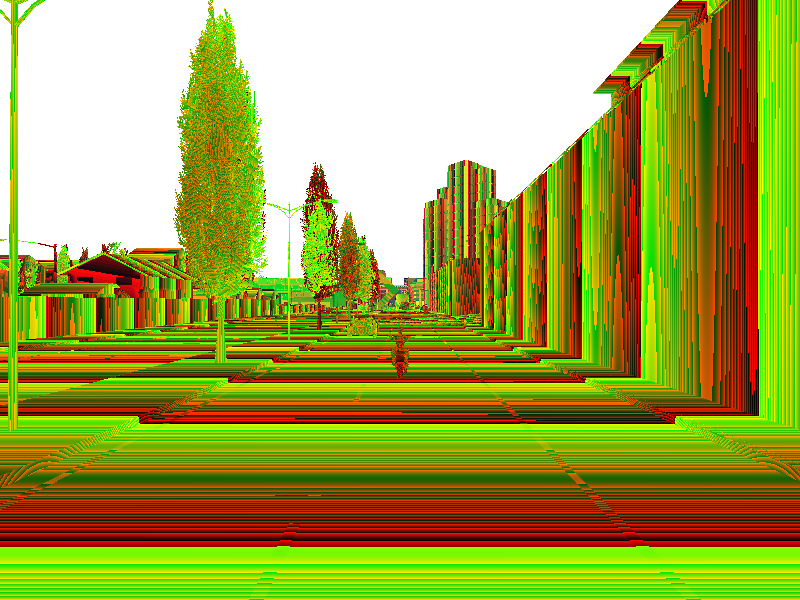
\includegraphics[width=0.4\textwidth]{depthimage.png}
	\caption{Depth image}
	\label{fig:depth image}
\end{figure}

This makes it possible to determine not only the direct distance of any visible object, but also the length of the object itself. By processing the calculated distance\,-\,vectors in a frame it is possible to estimate the length. To get accurate results at this early stage the object has to be fully visible. Otherwise the length is an approximated estimation. 
This value is added to the previously calculated distance to obtain the center of an object. To get the final position in the simulation environment taking into account the rotation of an object, the yaw\,-\,angle must be considered, too.\\


\subsubsection{Object Tracker}
Over time, new objects become visible and some disappear. For now, the detection algorithm can't track them. In addition, depending on the movement, objects are not detected in the same order. To keep track of all objects it is necessary to identify already detected ones in the following frames. To do so, all bounding boxes must get connected with an unique \ac{ID}. Also for this a function made available by pyimagesearch is used \cite{Tracker}. This Tracker was chosen for the reason that it is just necessary to provide coordinates of the bounding boxes. The code recognizes the movement and links an ID to a specific object in the bounding box.\\

%\subsubsection{Generating an object list}
%The results create an object list of transforms consisting of state\,-, dimension\,- and classification vectors of every detected object in the simulation using in\,-\,game camera sensors. This list can be compared to ground truth data directly coming from the simulation itself.\\